\documentclass{article}
\usepackage{graphicx}
\usepackage{alltt}
\usepackage{amsmath}
\usepackage{amsfonts}
\usepackage{bigstrut}
\usepackage{enumerate}
\usepackage{fancyhdr}
\usepackage[top=1.0in, bottom=1.5in, left=0.75in, right=0.75in]{geometry}
\usepackage{float}
\usepackage{lastpage}
\usepackage{tikz}
\usepackage[latin1]{inputenc}
\usepackage{color}
\usepackage{array}
\usepackage{longtable}
\usepackage{calc}
\usepackage{multirow}
\usepackage{hhline}
\usepackage{ifthen}
\usepackage{listings}
\usepackage{circuitikz}
\usepackage{caption}
\definecolor{mygreen}{rgb}{0,0.6,0}
\definecolor{mygray}{rgb}{0.5,0.5,0.5}
\definecolor{mymauve}{rgb}{0.58,0,0.82}
\lstset{ %
  backgroundcolor=\color{white},   % choose the background color; you must add \usepackage{color} or \usepackage{xcolor}; should come as last argument
  basicstyle=\normalsize,        % the size of the fonts that are used for the code
  breakatwhitespace=false,         % sets if automatic breaks should only happen at whitespace
  breaklines=true,                 % sets automatic line breaking
  captionpos=b,                    % sets the caption-position to bottom
  commentstyle=\color{mygreen},    % comment style
  deletekeywords={...},            % if you want to delete keywords from the given language
  escapeinside={\%*}{*)},          % if you want to add LaTeX within your code
  extendedchars=true,              % lets you use non-ASCII characters; for 8-bits encodings only, does not work with UTF-8
  frame=single,	                   % adds a frame around the code
  keepspaces=true,                 % keeps spaces in text, useful for keeping indentation of code (possibly needs columns=flexible)
  keywordstyle=\color{blue},       % keyword style
  language=python,                  % the language of the code
  morekeywords={*,...},            % if you want to add more keywords to the set
  numbers=left,                    % where to put the line-numbers; possible values are (none, left, right)
  numbersep=5pt,                   % how far the line-numbers are from the code
  numberstyle=\tiny\color{mygray}, % the style that is used for the line-numbers
  rulecolor=\color{black},         % if not set, the frame-color may be changed on line-breaks within not-black text (e.g. comments (green here))
  showspaces=false,                % show spaces everywhere adding particular underscores; it overrides 'showstringspaces'
  showstringspaces=false,          % underline spaces within strings only
  showtabs=false,                  % show tabs within strings adding particular underscores
  stepnumber=2,                    % the step between two line-numbers. If it's 1, each line will be numbered
  stringstyle=\color{mymauve},     % string literal style
  tabsize=2,	                   % sets default tabsize to 2 spaces
  title=\lstname                   % show the filename of files included with \lstinputlisting; also try caption instead of title
}
\floatstyle{boxed}
\floatstyle{plain}
\restylefloat{figure}
\pagestyle{fancy}
\fancyhead{}
\fancyfoot{}
\setlength{\headheight}{59.0pt}
\def\inputGnumericTable{}
\fancyhead[CO]{}
\lhead{\today}
\rhead{Page \thepage{} of \pageref{LastPage} }
\newlength\tindent
\setlength{\tindent}{\parindent}
\setlength{\parindent}{0pt}
\renewcommand{\indent}{\hspace*{\tindent}}

\usepackage[toc,page]{appendix}
\usepackage{titling}
\setlength{\droptitle}{-2.5cm}

\title{Air Force Institute of Technology \\ Department of Electrical and Computer Engineering}
\author{CSCE 654 - Computer Communication Networks \\ Project \#3 - Network Routing \\ \\ Author:  Micah Hayden }
\date{\today}

\begin{document}
\maketitle
%\begin{abstract}
%This is my abstract.
%\end{abstract}

\section{Introduction:}
\label{sec:Intro}

The goal of this project is to demonstrate the queuing impact of a routing network.
The network consists of 6 nodes A-F. 
All arrivals enter the system from the source into A at rate $\lambda$.
From there, messages are routed to their appropriate destination according to the network topology shown in Figure \ref{fig:Topology}.
The times shown along links between nodes A-F represent the propagation delays between nodes, while the percentages between a node and its sink represents the percentage of the total traffic, destined to the respective nodes. 
Node A has a service rate $\mu_A = 10 pps$, while all other nodes have service rate $\mu_{\bar{A}} = 20 pps$.

\begin{figure}[h!]
\centering
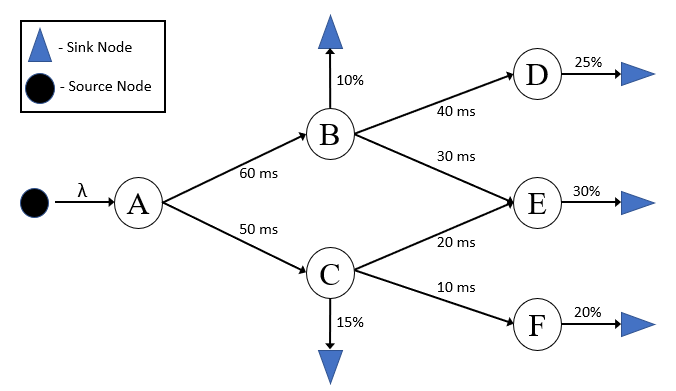
\includegraphics[scale=0.75]{Images/NetworkTopology.PNG}
\caption{Network Topology of Routing Network}
\label{fig:Topology}
\end{figure}

The key performance parameters for this experiment are the system delays - both per node, and the system as a whole; as well as the routing accuracy of the system.
Case 1 has a system arrival rate $\lambda_A = 15 \, pps$, and Case 2 has $\lambda_A = 17 \, pps$.

Mathematically analyzing the system prior to simulation allows prediction of the system response, as well as provides an anchor point for the results.
If the results match the expectation, the system functioned as expected.
However, if the results do not match, several questions arise:  was the simulation setup properly? Did the analysis not account for a particular parameter/factor?  
Was the particular queuing model used appropriate?

\section{Expected Results:}
\label{sec:ExpectedResults}
This section will go through the expected results of Case 1 \& Case 2.
The data to be analyzed is the routing accuracy and system delay, both per node and for the system as a whole.

The expected accuracy of the routing is simply the \% of packets routed to each destination.  Table \ref{tab:expTrafficLoad} below enumerates these expectations:

\begin{table}[h!]
\centering
\begin{tabular}{|c|c|} \hline
\textbf{Node} & \textbf{\% of Traffic} \\ \hline
A & 0 \\ \hline
B & 10 \\ \hline
C & 15 \\ \hline
D & 25 \\ \hline
E & 30 \\ \hline
F & 20 \\ \hline
Total & 100 \\ \hline
\end{tabular}
\caption{Expected traffic load per node}
\label{tab:expTrafficLoad}
\end{table}


Traffic with destination $E$ will be routed evenly through nodes $B$ and $C$.
This distributes the expected network traffic evenly across links $A \rightarrow B$ and $A \rightarrow C$, with each receiving $\frac{1}{2}$ of $E$'s traffic.\footnote{$Load_{link}$ is relative to the departure rate of the source node of the particular link.}

\begin{minipage}{.5\textwidth}
\begin{align*}
Load_{A \rightarrow B} 	&= Load_B + Load_D + \frac{1}{2} \cdot Load_E \\
						&= 0.10 + 0.25 + \frac{1}{2} \cdot 0.30 \\
						&= 0.50
\end{align*}
\vspace{.25cm}
\end{minipage}
\begin{minipage}{.5\textwidth}
\begin{align*}
Load_{A \rightarrow C} 	&= Load_C + Load_F + \frac{1}{2} \cdot Load_E \\
						&= 0.15 + 0.20 + \frac{1}{2} \cdot 0.30 \\
						&= 0.50
\end{align*}
\vspace{.25cm}
\end{minipage}

This shows that links $A \rightarrow B$ and $A \rightarrow C$ will each receive half of the traffic departing $A$.
Because $\mu_A > \lambda_A$, the $\text{Throughput}_A = \lambda_A$.
Thus, the arrival rate of nodes $B$ and $C$ equals $0.5 \cdot \lambda_A$.
Because $\mu_B = \mu_C = 10 \, pps$, and $10 \, pps > 0.5 \cdot \lambda_A$ for both cases, their throughput equals their arrival rates.  
In summary, because all queues in this system are stable, the throughput of any node equals the node's arrival rate.
It follows that any child node's arrival rate equals the percentage of the parent node's traffic that the child receives.
This yields the following arrival rates for cases 1 and 2.\footnote{$\lambda_E$ is the sum of its arrival rates from $B$ and $C$.}
\newline

\begin{minipage}{0.5\textwidth}
\centering
\begin{tabular}{|c|c|} \hline
\textbf{Node} & \textbf{Arrival Rate (pps)} \\ \hline
A & 15.0 \\ \hline
B & 7.5 \\ \hline
C & 7.5 \\ \hline
D & 3.75 \\ \hline
E & 4.5 \\ \hline
F & 3.0 \\ \hline
\end{tabular}
\captionof{table}{$\lambda$ for Case 1}
\label{tab:expArrival_case1}
\end{minipage}
\begin{minipage}{0.5\textwidth}
\centering
\begin{tabular}{|c|c|} \hline
\textbf{Node} & \textbf{Arrival Rate (pps)} \\ \hline
A & 17.0 \\ \hline
B & 8.5 \\ \hline
C & 8.5 \\ \hline
D & 4.25 \\ \hline
E & 5.1 \\ \hline
F & 3.4 \\ \hline
\end{tabular}
\captionof{table}{$\lambda$ for Case 2}
\label{tab:expArrival_case2}
\end{minipage}
\newline

With the arrival rates shown in Tables \ref{tab:expArrival_case1} and \ref{tab:expArrival_case2}, one can use Little's Law to calculate the expected time in the system, $E[r]$, for each node, using Equation \ref{eq:sysTime}.  
\begin{equation}
E[r] = \frac{1}{\mu - \lambda}
\label{eq:sysTime}
\end{equation}

Table \ref{tab:expSys} shows these times.
\newline

\begin{table}[h!]
\centering
\begin{tabular}{|c|c|c|} \hline
\textbf{Node} & \textbf{$\mathbf{E[r]}$ Case 1 (s)} & \textbf{$\mathbf{E[r]}$ Case 2 (s)} \\ \hline
A & 0.200 & 0.333 \\ \hline
B & 0.400 & 0.667 \\ \hline
C & 0.400 & 0.667 \\ \hline
D & 0.160 & 0.174 \\ \hline
E & 0.182 & 0.204 \\ \hline
F & 0.143 & 0.152 \\ \hline
\end{tabular}
\caption{Per-node system delays, $E[r]$}
\label{tab:expSys}
\end{table}

The times shown above indicate the time in the system \textbf{at} a particular node.
To find the expected system delay of a packet from source to its destination, one must also account for all nodes and propagation delays along its path.
For Node E, one must account for the separate paths to reach $E$.
Because half of its traffic goes through B and the other through C, this can be represented as the average system delay of 2 packets:  one going through B and the other through C to destination E.

This produces the following expected end-to-end delay (source to destination), for packets routed to each destination:

\begin{table}[h!]
\centering
\begin{tabular}{|c|c|c|} \hline
\textbf{Destination:} & \textbf{Case 1 Delay (s)} & \textbf{Case 2 Delay (s)} \\ \hline
B & 0.660 & 1.060 \\ \hline
C & 0.650 & 1.050 \\ \hline
D & 0.860 & 1.274 \\ \hline
E & 0.862 & 1.284 \\ \hline
F & 0.803 & 1.212 \\ \hline
\end{tabular}
\caption{Expected end-to-end delay by destination}
\label{tab:expEndDelay}
\end{table}

The overall network end-to-end delay is a weighted average of the values shown in Table \ref{tab:expEndDelay} with the expected Traffic Loads shown in Table \ref{tab:expTrafficLoad}.
This yields the following:
\newline

\begin{minipage}{0.5\textwidth}
\begin{align*}
\text{Network Delay}_{Case \, 1} = 0.798s
\end{align*}
\end{minipage}
\begin{minipage}{0.5\textwidth}
\begin{align*}
\text{Network Delay}_{Case \, 2} = 1.210s
\end{align*}
\end{minipage}
\newline 

\newpage
\section{Simulation Setup:}
\label{sec:SimSetup}

The basis of the omnet simulation was still the FIFO queue sample used for Project 2.
Each simulation run was 10 hours of sim-time.

\subsection{Routing:}
\label{subsec:RoutingSetup}
To accomplish the required routing, I utilized a custom message type \textbf{Netmsg}, which uses an integer to represent its destination.

I assigned each destination node a unique integer. \footnote{To account for the duplicate paths to node E, there were two integers for E, one for each path}.
The source node generates a random integer between 1 and 100, inclusive.  Based on the random number, it assigns a corresponding destination node.
As the number of messages grows, the distribution of destinations should approach the desired proportions.

The other modifications required were to detect whether a packet had arrived at its destination; and if not, to send it out on the appropriate link.
To accomplish this task, I modified the Fifo module's ``endService" function.
Previously, when the queue finished processing a packet, it immediately sent it out on the sole port.
The modifications change this to function to check if the packet's destination matches the queue's index.  
If so, the queue sends the packet to the sink node.
Otherwise, it uses simple logic to determine which of its outbound ports to send the message on.
The code for both of these operations are shown in Appendix \ref{appendix:SimFiles}.


\subsection{Network Configuration:}  
\label{subsec:Config}
I defined my network using an array of six FIFO queues and six sinks, as well as a single generator.
The connections account for the propagation delay on each link.
This topology matches that shown in Figure \ref{fig:Topology}.\footnote{There is a sink connected to A to ensure the simulator functioned properly, but is not shown on the network diagram.}


\subsection{Data Collection:}
\label{subsec:DataCollection}
There are several pieces of data which need to be collected during the simulation.
The first is the packet count at each sink, which will allow a comparison of each destination's traffic load.
Next is the packet lifetime.  
This statistic is used to compare the source-destination time for each packet.
Combined with the packet count, this will also allow the calculation of an overall network delay.

In order to properly analyze the system response to the network routing presented, I also need to collect data on each queues system time.
I modified the AbstractFifo.h and AbstractFifo.c files, which govern the FIFO queue nodes, by adding two new statistics:  serviceTime and nodeTime.
These values, in conjunction with the already-existing queueingTime statistic, will allow a comparison of the time spent at each node, and are collected immediately prior to sending the message from the queue to its destination.

\newpage
\section{Results \& Analysis:}
\label{sec:Results}
I conducted three simulations for each case, ensuring the results matched with different seeds and produced accurate results.
I collected data to compare the lifetime of packets at each node, as well as the total lifetime of the system.
The three runs were averaged for each case, producing the data used for the simulation analysis.

\subsection{Routing Accuracy \& Traffic Load:}
\label{subsec:RoutingResults}
To determine the routing accuracy and traffic load, I averaged the number of packets that arrived at each destination, relative to the total number of packets sent.

As seen in Figures \ref{fig:loadA} and \ref{fig:loadB}, my results closely matched the expected traffic load described in Table \ref{tab:expTrafficLoad}

\begin{minipage}{0.5\textwidth}
\centering
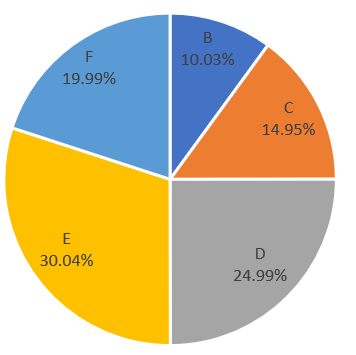
\includegraphics[scale=0.7]{Images/LoadA.PNG}
\captionof{figure}{Traffic Load with $\lambda_A = 15 \, pps$}
\label{fig:loadA}
\end{minipage}
\begin{minipage}{0.5\textwidth}
\centering
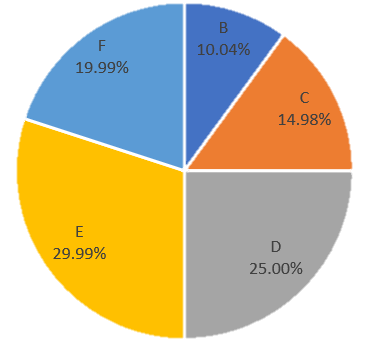
\includegraphics[scale=0.7]{Images/LoadB.PNG}
\captionof{figure}{Traffic Load with $\lambda_A = 17 \, pps$}
\label{fig:loadB}
\end{minipage}
\newline

The largest load difference was Case 1, with nodes C and E:  node C had $0.05\%$ less traffic than expected, while node E had $0.04\%$ more.\footnote{The raw data used to build Figures \ref{fig:loadA} and \ref{fig:loadB} is shown in Appendix \ref{appendix:Data}.}


\subsection{Per-Node System Times}
\label{subsec:systemTimes}
This section discusses how well each node performed, relative to the expected system times of Nodes A-F.
I used the \textbf{nodeTimeSignal} created for the FIFO nodes to measure the time spent at a given queue, to include the service time.
I then compared the simulation results to the expected nodal delays described in Table \ref{tab:expSys} in Section \ref{sec:ExpectedResults}.
Case 1 - $\lambda_A = 15$ pps - had an average difference of $0.343 \%$ from the expected nodal delays, while Case 2 - $\lambda_A = 17$ pps - had an average difference of $0.714\%$.
The data are shown in Tables \ref{tab:simNodeTimeA} and \ref{tab:simNodeTimeB} in Appendix \ref{appendix:Data}.
The accuracy of the simulation indicates that the the model utilized for this network matches the actual implementation.


\subsection{Network Delay:}
\label{subsec:NetworkDelay}
I used the statistics collected at each sink node to compare the per-destination average delay.
Both Case 1 and Case 2 performed well, with results closely matching the expectations.  
As expected, the largest end-to-end delays occurred when the destination was one of Nodes D-F. 
This occurs because to reach these destinations, they must go through two queue nodes, and two links before arriving at their destination's queue.
The per-destination end-to-end delays for Case 1 produced an average percent difference of $0.157\%$ from the expectation, while Case 2 had an average \% difference of $0.893\%$.\footnote{This \% difference simply averaged the \% differences for each destination's end-to-end delay, not based on the traffic load of each node.}

I calculated the network's average end-to-end delay for Cases 1 and 2 by using a weighted average of each destination's end-to-end delay, using the simulated traffic loads as the weight.

\begin{table}[h!]
\centering
\begin{tabular}{|c|c|c|c|} \hline
\textbf{Case \#} & \textbf{Simulated Delay (s)} & \textbf{Expected Delay (s)} & \textbf{\% Difference} \\ \hline
1 & 0.7992 & 0.7976 & 0.200 \\ \hline
2 & 1.1996 & 1.2095 & 0.822 \\ \hline
\end{tabular}
\caption{Average Network Delays}
\label{tab:lifetime}
\end{table}


The average network end-to-end delay for Case 1 was 0.7992 seconds, a $0.200 \%$ difference than the expected result.
The average end-to-end delay for Case 2 was 1.1996 seconds, a $0.822 \%$ difference than the expected result.
Figure \ref{fig:meanSysDelay} shows these results graphically, reinforcing the impact of the arrival rate on the long-term system response.


\begin{figure}[h!]
\centering
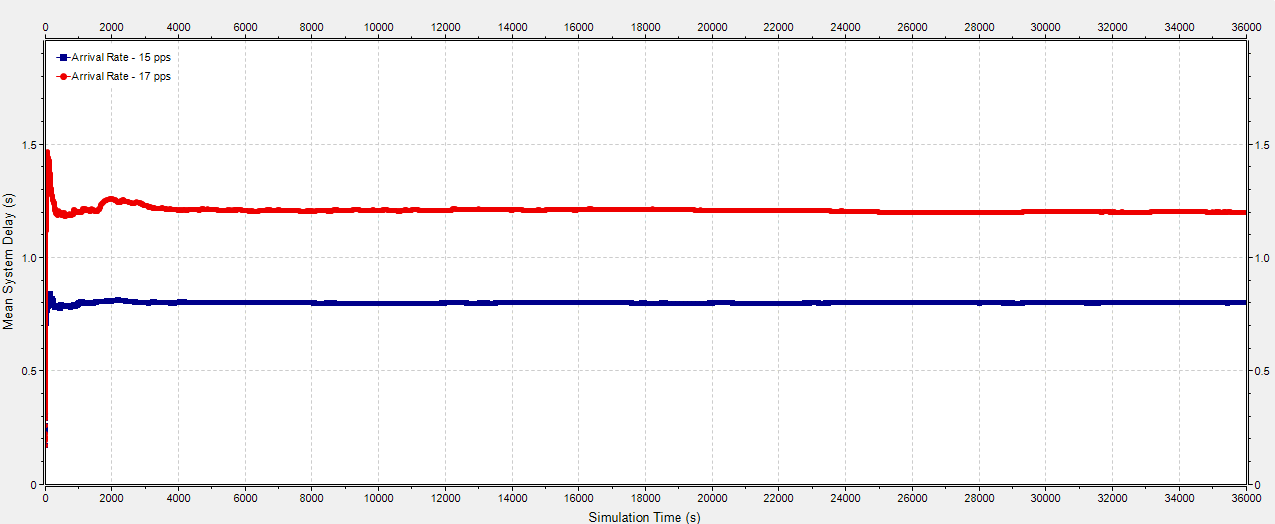
\includegraphics[scale=0.55]{Images/MeanSysDelay.PNG}
\caption{Mean System Delay}
\label{fig:meanSysDelay}
\end{figure}

Despite the difference in arrival rates, both cases produced a stable system.
However, change in arrival rate from 15 to 17 pps increased the expected delay by 0.4 seconds, a 50\% increase.


\subsection{Routing Decisions}
For my initial simulations, I used the assumption that splitting the traffic evenly between nodes B and C would produce the best overall system delay.
This assumption was used to calculate all expected results, and routed traffic to destination E evenly through B and C.
After seeing my results, I decided to run another round of simulations, routing a larger portion of the traffic through C, to see if the lower propagation delays experienced on that route would produce a correspondingly lower overall system delay.
Essentially, will the corresponding decrease in propagation time make up for the increase in queue time experienced on the route?
By routing more traffic through C, the traffic load at C would increase, causing increased queuing time for destinations C, E (through C), and F.  
However, it would also decrease the queue time experienced at destinations B, D, and E (through B) which have a higher total propagation time.

I ran two additional simulations, each with three trials.
Both simulations used an arrival rate of $\lambda_A = 17 \, pps$.
The first simulation used a small difference in the route selection to destination E:  routing 46.7\% of E's traffic through B, and sending the remaining 53.3\% through C.
This decision was made because the module generating destinations only used 1\% increments of the total traffic. 
Thus, the changes were from 15/15 to 14/16, and finally 10/20, where the values are the \% of total traffic.
Figure \ref{fig:unevenDelay} shows the results of these trials, compared to the simulation with an even distribution.

\begin{figure}[h!]
\centering
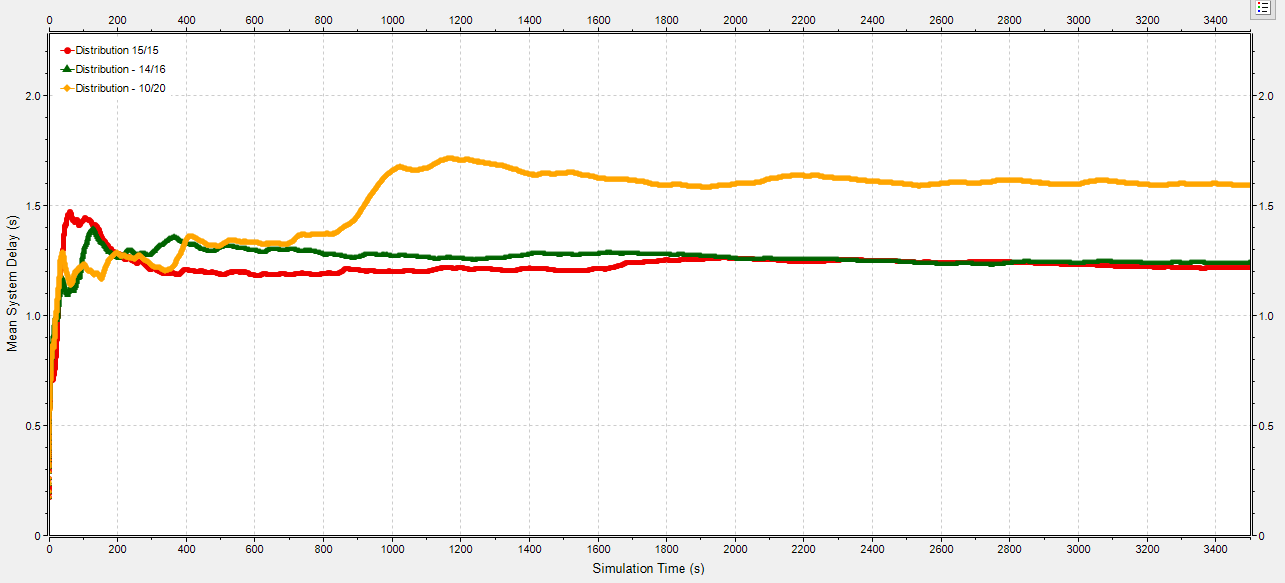
\includegraphics[scale=0.5]{Images/UnevenDist.PNG}
\caption{Network Delay with Uneven Routing to Destination E}
\label{fig:unevenDelay}
\end{figure}

The network delay of the original setup - with even routing had an average network delay of 1.1996 seconds.
The overall network delay for the small difference had an average network delay of 1.211 seconds, while the large difference had an average delay of 1.566 seconds, over a 10 hour simulation.

Based on these results, I am confident that the optimal distribution is to evenly distribute the traffic between B and C.
Any gains from reducing the propagation delay by $20 \, ms$ are negated by the corresponding increase in queue time.


\section{Conclusions:}
\label{sec:Conclusions}
This project worked as a functional model of simulated network traffic.
The traffic loads in simulation closely matched the desired network loads, with minor variations due to the probabilistic generation of destinations.
One can see the effects of the path length:  nodes D-F had a larger effect of propagation delay because they had to go through two paths.
On the other hand, nodes B and C only encounter a single propagation delay, on the path from node A.
Because all of the queues are stable, the throughput of a node $i$ is equivalent to the arrival rate $\lambda_i$.
This allows us to analyze the network as a sequence of M/M/1 queues because the interarrival times will still be exponentially distributed.
If queues B or C were unstable, destinations D-F would need further analysis to accurately model.




\newpage
\begin{appendices}
\section{Raw Data}
\label{appendix:Data}

\subsection*{Traffic Load}
\begin{minipage}{0.5\textwidth}
\centering
\begin{tabular}{|c|c|c|} \hline
\textbf{Node} & \textbf{Average Count} & \textbf{Percentage} \\ \hline
B & 54154 & 10.03 \\ \hline
C & 80705 & 14.95 \\ \hline
D & 134853 & 24.99 \\ \hline
E & 162120 & 30.04 \\ \hline
F & 107871 & 19.99 \\ \hline
\end{tabular}
\captionof{table}{Traffic Load for Case 1}
\label{tab:appTrafficA}
\end{minipage}
\begin{minipage}{0.5\textwidth}
\centering
\begin{tabular}{|c|c|c|} \hline
\textbf{Node} & \textbf{Average Count} & \textbf{Percentage} \\ \hline
B & 61412 & 10.04 \\ \hline
C & 91600 & 14.98 \\ \hline
D & 152887 & 25.00 \\ \hline
E & 183458 & 29.99 \\ \hline
F & 122293 & 19.99 \\ \hline
\end{tabular}
\captionof{table}{Traffic Load for Case 2}
\label{tab:appTrafficB}
\end{minipage}

\subsection*{Per-Node System Delay}
The following tables show the delay measured at each FIFO node in the system from the time a message entered a node's queue to the time it left its service.

\begin{table}[h!]
\centering
\begin{tabular}{|c|c|c|c|} \hline
\textbf{Node} & \textbf{Average Delay (s)} & \textbf{Expected Delay (s)} & \textbf{\% Difference} \\ \hline
A & 0.2008 & 0.2000 & 0.3958 \\ \hline
B & 0.3996 & 0.4000 & 0.0928 \\ \hline
C & 0.4006 & 0.4000 & 0.1541 \\ \hline
D & 0.1605 & 0.1600 & 0.2938 \\ \hline
E & 0.1833 & 0.1818 & 0.7876 \\ \hline
F & 0.1433 & 0.1429 & 0.3311 \\ \hline
\end{tabular}
\caption{System Delay for Nodes A-F with $\lambda_A = 15$ pps}
\label{tab:simNodeTimeA}
\end{table}

\begin{table}[h!]
\centering
\begin{tabular}{|c|c|c|c|} \hline
\textbf{Node} & \textbf{Average Delay (s)} & \textbf{Expected Delay (s)} & \textbf{\% Difference} \\ \hline
A & 0.3326 & 0.3333 & 0.2250 \\ \hline
B & 0.6516 & 0.6667 & 2.2587 \\ \hline
C & 0.6630 & 0.6667 & 0.5501 \\ \hline
D & 0.1738 & 0.1739 & 0.0400 \\ \hline
E & 0.2051 & 0.2041 & 0.4802 \\ \hline
F & 0.1504 & 0.1515 & 0.7313 \\ \hline
\end{tabular}
\caption{System Delay for Nodes A-F with $\lambda_A = 17$ pps}
\label{tab:simNodeTimeB}
\end{table}

\newpage
\subsection*{Per Destination End-to-End Delay}
\begin{table}[h!]
\centering
\begin{tabular}{|c|c|c|c|} \hline
\textbf{Destination} & \textbf{Average Delay (s)} & \textbf{Expected Delay (s)} & \textbf{\% Difference} \\ \hline
B & 0.660 & 0.660 & 0.007 \\ \hline
C & 0.651 & 0.650 & 0.144 \\ \hline
D & 0.861 & 0.860 & 0.105 \\ \hline
E & 0.865 & 0.862 & 0.383 \\ \hline
F & 0.806 & 0.803 & 0.410 \\ \hline
\textbf{Network:} & \textbf{0.799} & \textbf{0.798} & \textbf{0.200} \\ \hline
\end{tabular}
\caption{End-to-End Delays for Case 1}
\label{tab:nodeDelayA}
\end{table}

\begin{table}[h!]
\centering
\begin{tabular}{|c|c|c|c|} \hline
\textbf{Destination} & \textbf{Average Delay (s)} & \textbf{Expected Delay (s)} & \textbf{\% Difference} \\ \hline
B & 1.042 & 1.060 & 1.690 \\ \hline
C & 1.045 & 1.050 & 0.502 \\ \hline
D & 1.257 & 1.274 & 1.292 \\ \hline
E & 1.277 & 1.284 & 0.585 \\ \hline
F & 1.207 & 1.212 & 0.397 \\ \hline
\textbf{Network:} & \textbf{1.120} & \textbf{1.210} & \textbf{0.822} \\ \hline
\end{tabular}
\caption{End-to-End Delays for Case 2}
\label{tab:nodeDelayB}
\end{table}

\newpage
\section{Simulation Files}
\label{appendix:SimFiles}

\begin{figure}[h!]
\begin{lstlisting}
[General]
network = Network_Forward
sim-time-limit = 10h
cpu-time-limit = 300s
#debug-on-errors = true
#record-eventlog = true

[Config NetworkA]
description = "Arrival rate of 15 pps"
repeat = 3
**.gen.sendIaTime = 	 exponential(0.06667s)
**.fifo[0].serviceTime = exponential(0.05s)
**.fifo[1].serviceTime = exponential(0.1s)
**.fifo[2].serviceTime = exponential(0.1s)
**.fifo[3].serviceTime = exponential(0.1s)
**.fifo[4].serviceTime = exponential(0.1s)
**.fifo[5].serviceTime = exponential(0.1s)

[Config NetworkB]
description = "Arrival rate of 17 pps"
repeat = 3
**.gen.sendIaTime = 	 exponential(0.05882s)
**.fifo[0].serviceTime = exponential(0.05s)
**.fifo[1].serviceTime = exponential(0.1s)
**.fifo[2].serviceTime = exponential(0.1s)
**.fifo[3].serviceTime = exponential(0.1s)
**.fifo[4].serviceTime = exponential(0.1s)
**.fifo[5].serviceTime = exponential(0.1s)
\end{lstlisting}
\vspace{-1cm}
\caption*{Simulation Initialization File - omnetpp.ini}
\end{figure}

\begin{figure}[h!]
\begin{lstlisting}
network Network_Forward
{
    @display("bgb=564,468");
    submodules:
        gen: Source {
            parameters:
                @display("p=45,136");
        }
        fifo[6]: Fifo {
            @display("p=239,136,c");
        }
        sink[6]: Sink {
            @display("p=427,136,c");
        }
    // fifo[1]-fifo[5] correspond to fifoB --> fifoF
    connections:
        gen.out --> fifo[0].in++;
        fifo[0].out++ --> {  delay = 60 ms; } --> fifo[1].in++;
        fifo[0].out++ --> {  delay = 50 ms; } --> fifo[2].in++;
        fifo[1].out++ --> {  delay = 40 ms; } --> fifo[3].in++;
        fifo[1].out++ --> {  delay = 30 ms; } --> fifo[4].in++;
        fifo[2].out++ --> {  delay = 20 ms; } --> fifo[4].in++;
        fifo[2].out++ --> {  delay = 10 ms; } --> fifo[5].in++;

        // Output gates to sinks:
        fifo[0].sink --> sink[0].in;
        fifo[1].sink --> sink[1].in;
        fifo[2].sink --> sink[2].in;
        fifo[3].sink --> sink[3].in;
        fifo[4].sink --> sink[4].in;
        fifo[5].sink --> sink[5].in;

}
\end{lstlisting}
\vspace{-1cm}
\caption*{Network Description (NED) File}
\end{figure}

\begin{figure}[h!]
\begin{lstlisting}
void Fifo::endService(cMessage *msg)
{
    EV << "Completed service of " << msg->getName() << endl;
    int dest = check_and_cast<Netmsg *>(msg)->getDestination();
    // At destination:
    if (getIndex() == dest) {
        send(msg, "sink");
    }
    // At E from C
    else if (getIndex() == 4 && dest == 44 ) {
        send(msg, "sink");
    }
    // At A:
    else if (getIndex() == 0) {
        if (dest == 1 || dest == 3 || dest == 4)
            send(msg, "out", 0);
        else {
            send(msg, "out", 1);
        }
    }
    // At B:
    else if (getIndex() == 1) {
        if (dest == 3) {
            send(msg, "out", 0);
        }
        else {
            send(msg, "out", 1);
        }
    }
    // At C:
    else if (getIndex() == 2) {
        if (dest == 44) {
            send(msg, "out", 0);
        }
        else {
            send(msg, "out", 1);
        }
    }
}
\end{lstlisting}
\vspace{-1cm}
\caption*{FIFO endService Function}
\end{figure}

\begin{figure}[h!]
\begin{lstlisting}
void Source::handleMessage(cMessage *msg)
{
    ASSERT(msg == sendMessageEvent);

    Netmsg *job = new Netmsg("job");
    // Produce source and destination address using probabilities.
    int probDest = intuniform(1, 100);
    int dest;
    if (probDest <= 10) {
        // Destination = B
        dest = 1;
    }
    else if (probDest <= 25) {
        // Destination = C
        dest = 2;
    }
    else if (probDest <= 50) {
        // Destination = D
        dest = 3;
    }
    else if (probDest <= 65) { //--> Using below probability to test uneven distribution through B/C
    //else if (probDest <= 60) {
        // Destination = E --> Send through B
        dest = 4;
    }
    else if (probDest <= 80) {
        // Destination = E --> Send through C
        dest = 44;
    }
    else {
        // Destination = F
        dest = 5;
    }
    job->setDestination( dest );
    send(job, "out");

    scheduleAt(simTime()+par("sendIaTime").doubleValue(), sendMessageEvent);
}
\end{lstlisting}
\vspace{-1cm}
\caption*{Source Node - destination logic}
\end{figure}

\begin{figure}[h!]
\begin{lstlisting}
namespace fifo;

message Netmsg {
    int destination;
}
\end{lstlisting}
\vspace{-1cm}
\caption*{Netmsg Type}
\end{figure}

\end{appendices}

\end{document}
